\documentclass[20pt]{article}

\usepackage{hyperref}
\hypersetup{
    colorlinks=true,
    linkcolor=blue,
    filecolor=magenta,
    urlcolor=cyan,
    pdftitle={Dreamcast},
    pdfpagemode=FullScreen,
    }

\usepackage{graphicx}
\graphicspath{ {./images/} }

\title{Dreamcast JVM}
\date{}

\setcounter{secnumdepth}{0}

\begin{document}

\maketitle
%\href{images/revision-1-inserted.png}{\includegraphics{images/revision-1-inserted.png}}

\tableofcontents
\section{Introduction}

This is a from-scratch JVM implementation for Sega Dreamcast, from zero to
3D spinning translucent textured cubes in 14 days.

This is not a port of the JVM from the OpenJDK project, but instead a completely
separate and independent implementation that follows the same specification.

My time on this project was split roughly 3 ways:

\begin{itemize}
\item 30\% of my time was spent writing the actual JVM itself

\item 30\% on writing new Java libraries for manipulating the Dreamcast hardware

\item 30\% on writing a "load Java classes the Dreamcast GDROM drive" loader.

\item 10\% on designing Java APIs, (and reviewing existing APIs, e.g:
  \texttt{java.nio}/\texttt{sun.misc}), particularly related to giving Java code
  direct and arbitrary access to Dreamcast memory/registers
\end{itemize}

\section{Demo download}

There are three different versions of my demo, depending on how/where you'd like
to run this:

\subsection{Dreamcast (for physical CD-R; may also work on GD-ROM drive emulators)}
\begin{itemize}
\item \href{https://dreamcast.idk.st/jvm/jvm-cube-dreamcast.cdi}{jvm-cube-dreamcast.cdi}
\end{itemize}

\subsection{Dreamcast (for loading via a Dreamcast USB-UART)}
\begin{itemize}
\item \href{https://dreamcast.idk.st/jvm/jvm-cube-usb-uart.bin}{jvm-cube-usb-uart.bin}
\end{itemize}

\subsection{Flycast}
\begin{itemize}
\item \href{https://dreamcast.idk.st/jvm/jvm-cube-flycast.cdi}{jvm-cube-flycast.cdi}
\end{itemize}

\section{Current status}

The current Dreamcast JVM implementation is fairly complete, and will correctly
interpret a wide range of Java code correctly.

However, the following JVM features are not supported:

\begin{itemize}
\item exceptions (\texttt{try}/\texttt{catch}/\texttt{finally} in Java)

\item separately from the above, \texttt{finally} clauses from Java versions <=1.4 (2002 or
  earlier)

\item \texttt{invokedynamic} (Java lambdas, Java string concatenation, etc...)

\item \texttt{synchronized} methods (Java threads are also not implemented)

\item runtime type checks (\texttt{instanceof}/\texttt{checkedcast}) on
  zero-length/null arrays of references

\item garbage collection and memory deallocation (technically not required of a
  JVM, but fair to expect of a JVM that this exists)
\end{itemize}

The above list is \textit{probably} exhaustive. An attempt to do any of these
will trigger a failed assertion, and JVM execution will halt.

Other than above list, generally speaking Java class files emitted by any Java
version from 6 through 23 inclusive should be compatible with the Dreamcast JVM.

\section{How much of this cube demo is written in Java?}

To the greatest extent that Java (a language that does not have memory address
dereferences as a built-in language construct) is able, all manipulations of
Dreamcast hardware and memory state are manipulated directly from Java
code. Memory access occurs either directly via the \texttt{Memory.getU4} and
\texttt{Memory.putU4} static methods, or indirectly via the Dreamcast DMA
controllers.

There are no “foreign calls” to C libraries whatsoever.

The cube demo is 100\% native Java.

\section{How does the demo work?}

I believe it could be interesting if it were possible to author code for the
Dreamcast without GCC/binutils. In service to this idea, I designed this
multi-stage “boot” process. The boot process allows Java class files to be
automatically loaded from iso9660 on a CD, rather than embedded in another
binary file via a specialized toolchain.

This means that anyone with a generic \texttt{javac}, \texttt{mkisofs}, and
copies of \texttt{jvm.bin} and \texttt{gdrom\_jvm\_boot.bin} can write code for
the Dreamcast.

\href{boot.svg}{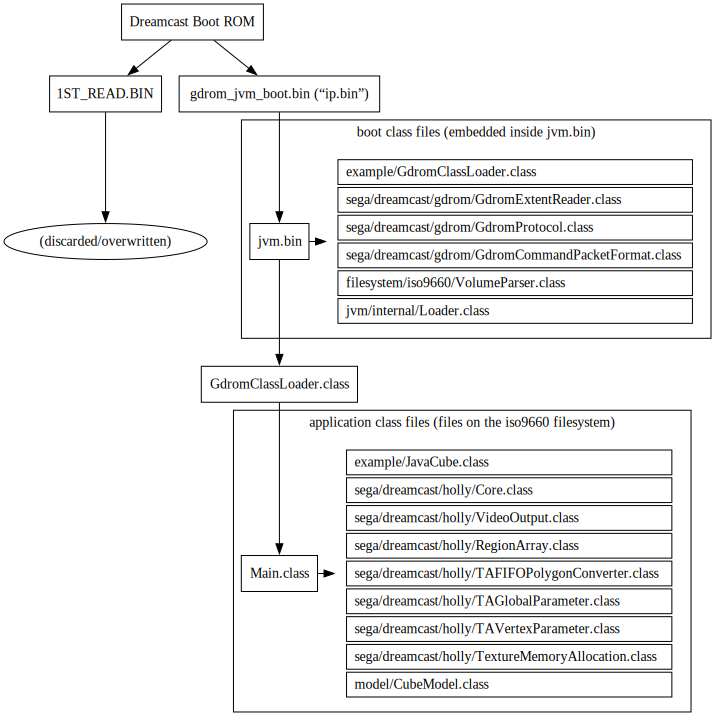
\includegraphics{boot.svg}}

\section{Could the Dreamcast JVM also work on Sega Saturn?}

\textbf{Yes.}

Java float and double primitives are perhaps the only obstacle.

Though the JVM specification does clearly specify that float and double
\textbf{must} be in IEEE-754 format, I think it would be interesting to instead
implement float as 16.16 fixed-point, and double as 32.32 fixed-point on Saturn
in deliberate violation of the specification.

Implementing fixed-point operations as primitive types rather than as a
“FixedPoint” class in Java would also yield significantly better
performance---arithmetic opcode execution is practically "free" compared to the
expense of resolving and calling instance methods, not even considering the
additional pointer indirections.

\section{What about JVM languages other than Java?}

Kotlin “hello world” works in the current Dreamcast JVM implementation:

\begin{verbatim}
fun main() {
  println("Hello world!")
}
\end{verbatim}

I did not test beyond this.

The most probable issue with attempts to run Kotlin/Clojure/Jython, etc... (and
in particular their interpreters) on the Dreamcast JVM is most of the Java SE
class library is missing. This is not a hard issue to solve; perhaps just
slightly tedious at worst.

\section{Why can't you just use the Java SE libraries from OpenJDK with the Dreamcast JVM?}

The OpenJDK class libraries depend on the OpenJDK JVM's internals (for which
there is no formal specification).

\section{What about performance? Is the Dreamcast JVM fast?}

\textbf{Absolutely not.}

On the current JVM implementation, expect performance
somewhere on the order of \textbf{100x slower} than semantically-equivalent C
code as compiled by GCC.

The fact that my cube demo spins at all at relatively nice-looking framerates is
a testament to the brute speed of the SH7091 SH4 CPU in the Dreamcast.

\section{Could Dreamcast JVM performance improve?}

The Dreamcast JVM is a fairly naive bytecode interpreter, so there are myriad
ways to improve performance. For long sequences of arithmetic operations (e.g: a
vertex transformation function), it is fairly obvious that the solution should
be to JIT-compile the bytecodes to SH instructions. I think this should be
fairly easy to do.

While there have been several "JIT-compile SH to x86" projects (as in Dreamcast
emulators), I am not aware of any "JIT-compile [thing] to SH" projects. This
adds to the list of reasons why I think this would be interesting to pursue.

Indepent of bytecode execution: method lookups, and particularly instance method
lookups, are slower than they could be. Perhaps in parallel with the JIT effort,
with a more thorough “linking” process, method lookups could likely become about
as fast as calling a function pointer in C.

\section{Does this mean Java ME games for early 2000's mobile phones could be run on Dreamcast?}

I like this idea. Unlike Java SE, which is fairly huge, implementing the Java ME
class libraries feels closer to what could be a one-person initiative.

It could also be fun to implement the "Mobile 3D Graphics" Java ME profiles for
Dreamcast.

\section{What about .NET/CLR for Dreamcast/Saturn?}

The Dreamcast JVM project would not have been possible without the excellent and
freely-available specification:

\href{https://docs.oracle.com/javase/specs/jvms/se23/html/index.html}{https://docs.oracle.com/javase/specs/jvms/se23/html/index.html}

I am aware that a CLR/CLI/CIL specification exists as well:

\href{https://ecma-international.org/wp-content/uploads/ECMA-335_6th_edition_june_2012.pdf}{https://ecma-international.org/wp-content/uploads/ECMA-335\_6th\_edition\_june\_2012.pdf}

The ECMA-335 specification looks fairly complete/implementable, and I estimate
such a project would be roughly on the same level of effort as this JVM project.

I don't know. Maybe?

\section{Other possible future directions}

I am interested in hearing anyone's opinions on any topic even vaguely related
to any of the above.

\end{document}
